
%(BEGIN_QUESTION)
% Copyright 2006, Tony R. Kuphaldt, released under the Creative Commons Attribution License (v 1.0)
% This means you may do almost anything with this work of mine, so long as you give me proper credit

The following water heater process is automated with a pneumatic temperature transmitter, controller, and control valve:

$$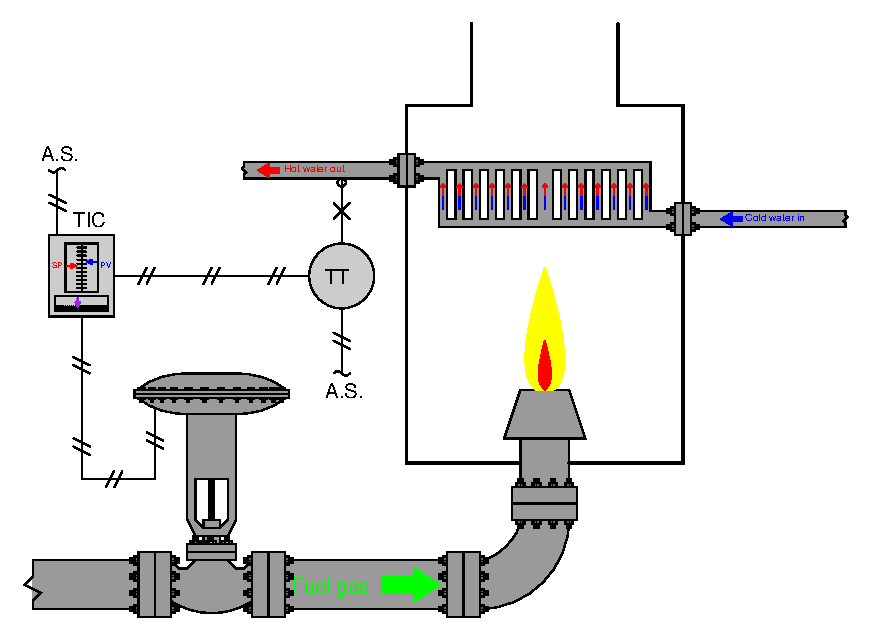
\includegraphics[width=15.5cm]{i01460x01.eps}$$

The process variable (PV), setpoint (SP), and output signals (manipulated variable, or MV) of the controller are recorded in a table at random time intervals:

% No blank lines allowed between lines of an \halign structure!
% I use comments (%) instead, so that TeX doesn't choke.

$$\vbox{\offinterlineskip
\halign{\strut
\vrule \quad\hfil # \ \hfil & 
\vrule \quad\hfil # \ \hfil & 
\vrule \quad\hfil # \ \hfil \vrule \cr
\noalign{\hrule}
%
% First row
PV & SP & MV \cr
%
(Process Variable) & (Setpoint) & (Output) \cr
%
\noalign{\hrule}
%
% Another row
50\% & 50\% & 50\% \cr
%
\noalign{\hrule}
%
% Another row
45\% & 50\% & 55\% \cr
%
\noalign{\hrule}
%
% Another row
30\% & 50\% & 70\% \cr
%
\noalign{\hrule}
%
% Another row
25\% & 50\% & 75\% \cr
%
\noalign{\hrule}
%
% Another row
65\% & 50\% & 35\% \cr
%
\noalign{\hrule}
%
% Another row
72\% & 50\% & 28\% \cr
%
\noalign{\hrule}
%
% Another row
50\% & 40\% & 40\% \cr
%
\noalign{\hrule}
%
% Another row
50\% & 71\% & 71\% \cr
%
\noalign{\hrule}
%
% Another row
80\% & 65\% & 35\% \cr
%
\noalign{\hrule}
%
% Another row
37\% & 42\% & 55\% \cr
%
\noalign{\hrule}
%
% Another row
40\% & 30\% & 40\% \cr
%
\noalign{\hrule}
} % End of \halign 
}$$ % End of \vbox

Develop a mathematical expression describing the data you see here in the table.  Hint: it may be easier if you begin with a {\it qualitative} assessment of the figures (i.e. {\it ``when the PV exceeds the SP, the MV . . .''}).

\underbar{file i01460}
%(END_QUESTION)





%(BEGIN_ANSWER)

MV = SP $-$ PV + 50\%

%(END_ANSWER)





%(BEGIN_NOTES)


%INDEX% Control, proportional: controller gain

%(END_NOTES)


